\subsection{Méthodologie}
\label{subsec:stabilite_methode}

L'analyse de la stabilité de la fusée SP-02 a été réalisée en utilisant deux outils principaux : \gls{Stabtraj} et \gls{OpenRocket}. Ces
logiciels permettent de modéliser la fusée, d'analyser ses caractéristiques aérodynamiques et de simuler son comportement en vol. La
méthodologie suivie pour l'analyse de la stabilité comprend les étapes suivantes:\\

\begin{enumerate}
    \item \textbf{Modélisation \acrshort{CAO} :} La fusée SP-02 a été modélisée en détail dans un logiciel de \acrshort{CAO}, en tenant
    compte des dimensions, de la géométrie et de la répartition des masses de chaque composant.\\
    
    \item \textbf{Importation dans \gls{OpenRocket} :} Après avoir finalisé la modélisation \acrshort{CAO}, le modèle a été construit dans
    le logiciel \gls{OpenRocket} à partir de ces brics de construction. Cette étape permet essentiellement de placer les différents éléments
    de la fusée et de leur attribuer des matériaux. Cela permet de définir la masse et le \acrfull{CdG} de chaques éléments et donc de
    la fusée dans son ensemble. Aussi, \gls{OpenRocket} permet d'estimer les caractéristiques aérodynamiques de la fusée, telles que le
    coefficient de traînée ($C_d$), le coefficient de portance ($C_l$) et le \acrfull{CdP}, en fonction de la géométrie et des conditions
    de vol.\\

    \item \textbf{Importation dans \gls{Stabtraj} :} Le modèle de la fusée a ensuite été importé dans \gls{Stabtraj} en comptant la masse et
    le \acrshort{CdG} ainsi que le $C_d$ fournis par \gls{OpenRocket}. En utilisant ces données, \gls{Stabtraj} permet de calculer le
    \acrshort{CdP} à partir de l'approximation de Barrowman \cite{Stab_doc} et d'analyser la stabilité longitudinale de la fusée.\\

    \item \textbf{Correction et itérations :} Si les résultats de l'analyse de stabilité indiquent que la fusée n'est pas stable, des
    ajustements sont effectués sur la conception, tels que le déplacement du \acrshort{CdG} ou la modification de la géométrie des surfaces
    de portances. La nouvelle conception est ensuite réévaluée en répétant les étapes précédentes jusqu'à obtenir une stabilité
    satisfaisante.\\
\end{enumerate}

\vfill

\begin{figure}[h!]
    \centering
    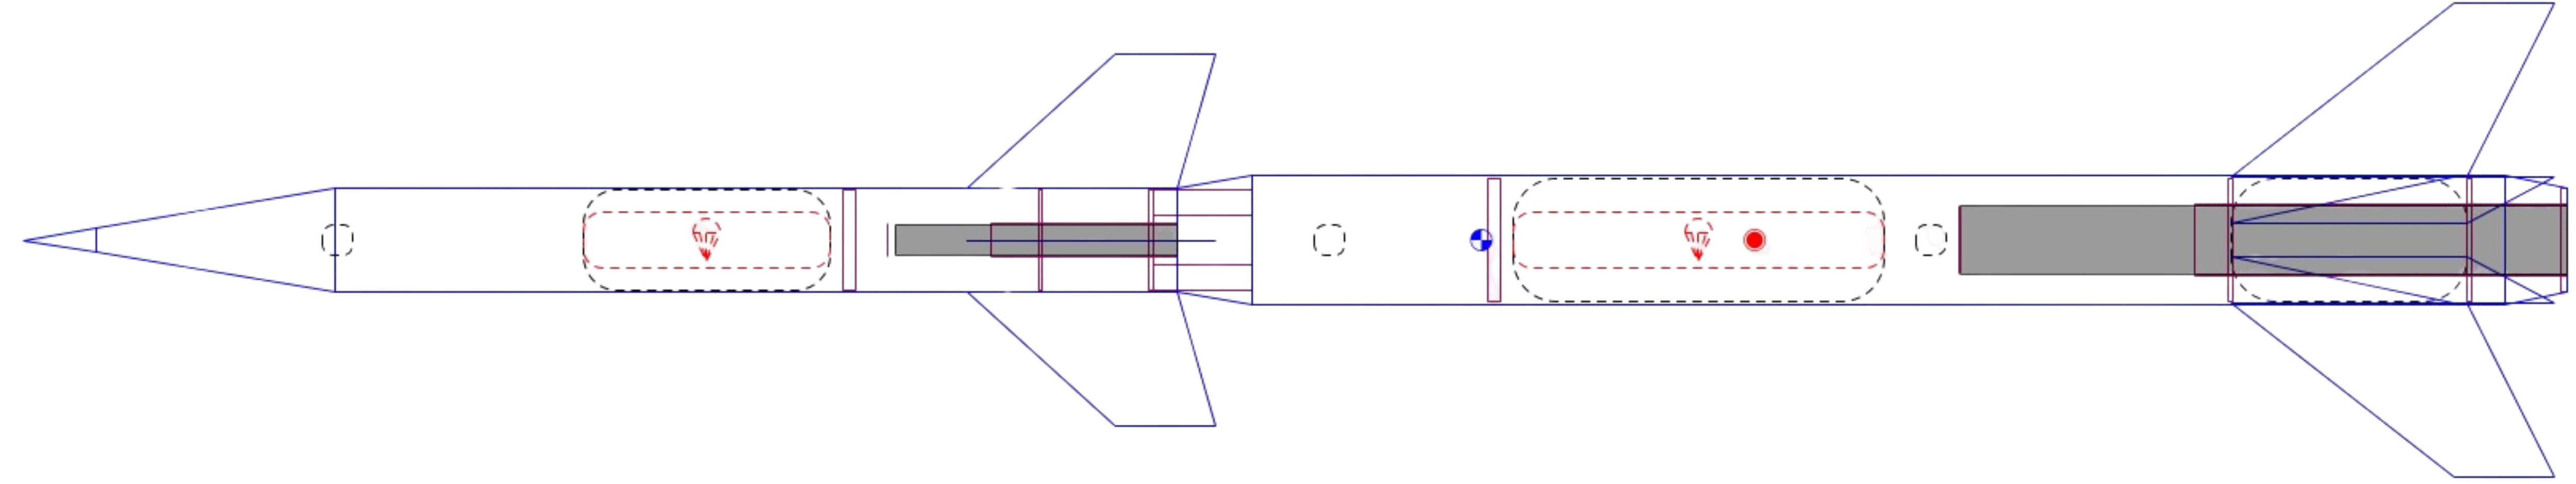
\includegraphics[width=\textwidth]{figures/sp02_ork.png}
    \caption{Modélisation de la fusée SP-02 dans \gls{OpenRocket}}
    \label{fig:sp02_ork_model}
\end{figure}

\vfill

\newpage
